\chapter{Fundamentação teórica}

    Este capítulo apresenta os fundamentos teóricos que embasam o desenvolvimento do sistema automatizado proposto. São abordados inicialmente aspectos conceituais e técnicos sobre piscinas e seus processos de manutenção, contemplando histórico, estrutura e procedimentos de limpeza manual e química. Em seguida, discorrem-se os princípios da automação residencial, destacando sua evolução, principais componentes e tecnologias aplicáveis. Essa base teórica é essencial para compreender as decisões tomadas para a construção do trabalho e a metodologia de implementação adotada nos capítulos seguintes.

\section{PISCINAS e sua manutenção}

    A compreensão dos processos de automação voltados à limpeza e manutenção de piscinas requer, primeiramente, o entendimento de sua estrutura física, funcionamento e métodos tradicionais de conservação da qualidade da água. Este tópico apresenta um panorama sobre o surgimento e a popularização das piscinas, seus componentes essenciais, bem como as técnicas manuais e químicas de limpeza empregadas para assegurar a salubridade e o equilíbrio químico da água. Essas informações fornecem o suporte técnico necessário para fundamentar a proposta de automação apresentada posteriormente.

    \subsection{HISTÓRICO E POPULARIZAÇÃO DAS PISCINAS}
    
        O termo piscina, que vem do latim piscis (“peixe”), pode ser definido como um tanque cheio de água destinado a diversos fins, sejam eles natação, mergulho, saltos ornamentais ou simplesmente recreação\cite{piscinaOquee}. Há registros de piscinas desde 2600 a.C., como “Os Grandes Banhos de Mohenjodaro”, considerado um dos primeiros tanques públicos de água, construído em tijolos e revestido com gesso. Contudo, acredita-se que esse tanque tenha sido feito apenas para fins religiosos.
         \begin{figure}[H]
         	\centering
         	\caption{ }  
        	\centering
         	\label{fig:cont}
        	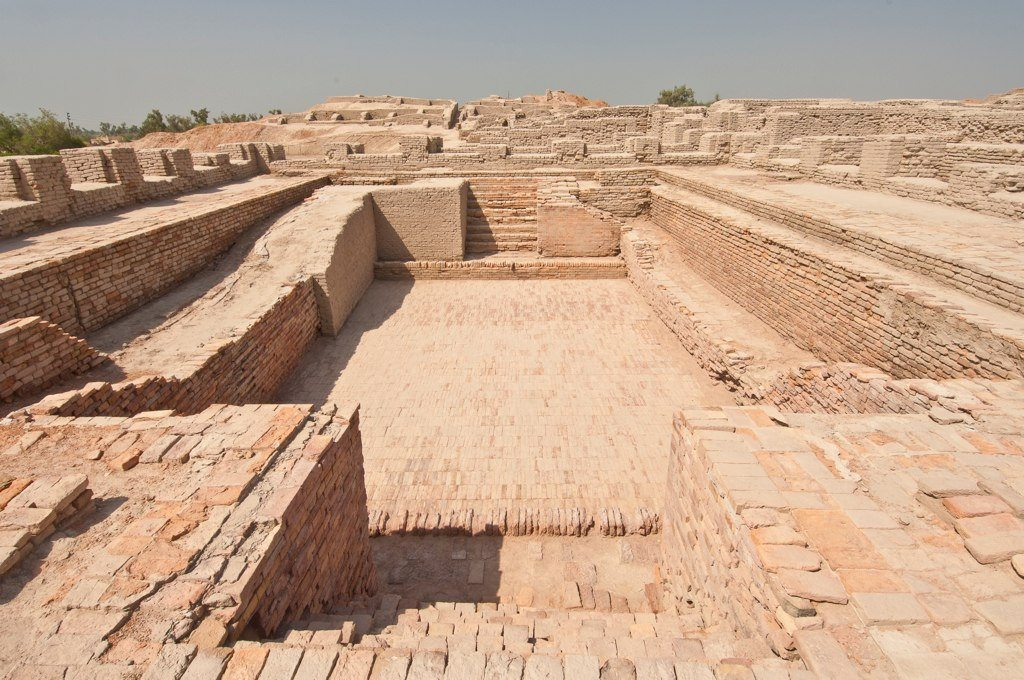
\includegraphics[width=0.78\textwidth]{imagens/primeiraPiscina.png}
        	\caption*{Fonte: \cite{piscinaHistoria}}
         \end{figure}
        
        Com o avanço da tecnologia no século XX, as piscinas passaram a incorporar novos sistemas, como os de cloração e filtração, que permitiram manter a água limpa sem a necessidade de trocas completas, prática que antes era essencial. No Ocidente, as piscinas começaram a se popularizar com a invenção do gunite (mistura de cimento, areia e água), um material que facilitava a instalação, possibilitava projetos mais flexíveis e reduzia consideravelmente o custo de construção\cite{piscinaHistoria}.

    \subsection{COMPONENTES BÁSICOS DE UMA PISCINA}
        
        \textcolor{black}{De acordo com \cite{refComponents}, as piscinas podem ser compreendidas, de forma conceitual, como estruturas simples destinadas ao armazenamento de grandes volumes de água para uso recreativo. Podem apresentar diferentes tipologias, como piscinas de ondas em parques aquáticos, particulares ou públicas, entre outras. No entanto, de modo geral, todas compartilham componentes fundamentais que asseguram o adequado processo de filtração e tratamento químico da água.}

        \textcolor{black}{Diante disso, torna-se essencial compreender os principais componentes estruturais de uma piscina, os quais garantem o funcionamento adequado do sistema de circulação e tratamento da água. Entre eles, destacam-se a bomba motorizada, o filtro de água, o alimentador químico, os drenos, as devoluções e os encanamentos de PVC\footnote{Sigla para Poli(cloreto de vinila), um polímero termoplástico versátil, conhecido por sua durabilidade, resistência química e ampla utilização em tubos, conexões e revestimentos.}. Em algumas instalações, inclui-se ainda um aquecedor, cuja função é manter a temperatura da água em níveis controlados e confortáveis.}

        \begin{itemize}
        
            \item \textcolor{black}{Bomba Motorizada:}
                \textcolor{black}{Responsável por circular toda a água, puxando-a da bacia e conduzindo-a até os demais processos.}

            \item \textcolor{black}{Filtro de Água:}
                \textcolor{black}{Remove parte das impurezas da água, como folhas, poeira e micro-organismos.}

            %\item \textcolor{black}{Alimentador Químico:}
                %\textcolor{black}{Distribui os produtos químicos responsáveis pela limpeza e manutenção da qualidade da água.}

            \item \textcolor{black}{Drenos:}
                \textcolor{black}{Removem a água utilizada em processos de limpeza, escoamento ou manutenção.}

            \item \textcolor{black}{Devoluções:}
                \textcolor{black}{Pontos de reabastecimento da água na piscina.}

            \item \textcolor{black}{Encanamentos de PVC:}
                \textcolor{black}{Interligam todos os componentes da piscina, permitindo o transporte adequado da água.}
                %Colocar uma imagem de cada item respectivo ou uma no final que tenha todos
                
        \end{itemize}

        \begin{figure}[H]
         	\centering
         	\caption{ }  
        	\centering
         	\label{fig:cont}
        	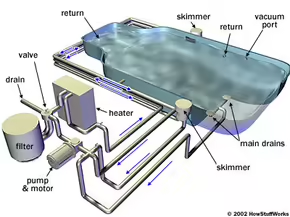
\includegraphics[width=0.48\textwidth]{imagens/componentesPiscina.png}
            \caption*{Componentes básicos de uma piscina}
        	\caption*{Fonte: \cite{refComponents}}
         \end{figure}

        \textcolor{black}{Todos esses componentes têm como finalidade manter a circulação da água em um ciclo contínuo, conduzindo-a por todo o sistema de filtração e tratamento químico. Além disso, há dispositivos complementares destinados a auxiliar na limpeza física da piscina, os quais serão detalhados nas seções seguintes.}

        \subsubsection*{Aspirador de escova}

         \textcolor{black}{Segundo \cite{benedito2024projeto}, o aspirador de escova é um dos itens mais importantes na limpeza física da piscina, tendo como função a aspiração da sujeira acumulada no fundo.}

            \begin{figure}[H]
                \centering
                \caption{ }  
                \centering
                \label{fig:cont}
                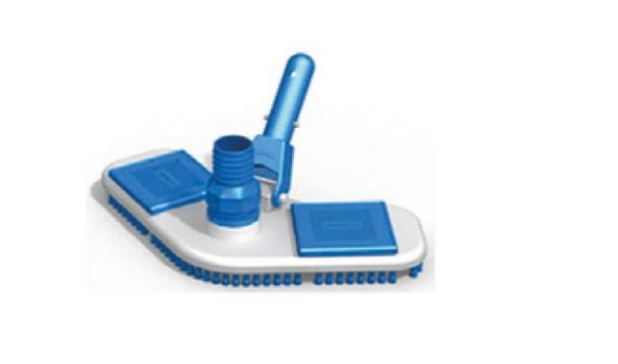
\includegraphics[width=0.60\textwidth]{imagens/aspirador.png}
                \caption*{Aspirador de escova}
                \caption*{Fonte: \cite{benedito2024projeto}}
            \end{figure}

        \subsubsection*{Peneira}

         \textcolor{black}{A peneira é responsável pela coleta de resíduos, como insetos, plásticos e pequenas folhas que ficam flutuando na superfície da piscina \cite{benedito2024projeto}.}

            \begin{figure}[H]
                \centering
                \caption{ }  
                \centering
                \label{fig:cont}
                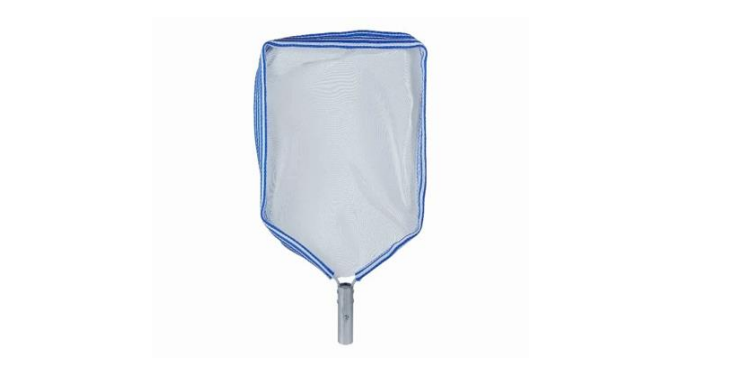
\includegraphics[width=0.60\textwidth]{imagens/peneira.png}
                \caption*{Peneira}
                \caption*{Fonte: \cite{benedito2024projeto}}
            \end{figure}

        \subsubsection*{Escova}

         \textcolor{black}{De acordo com o \cite{benedito2024projeto}, a escova é um dos principais equipamentos utilizados na limpeza da piscina. É responsável pela remoção de poeira e algas das paredes, podendo também ser utilizada na limpeza do fundo.}

            \begin{figure}[H]
                \centering
                \caption{ }  
                \centering
                \label{fig:cont}
                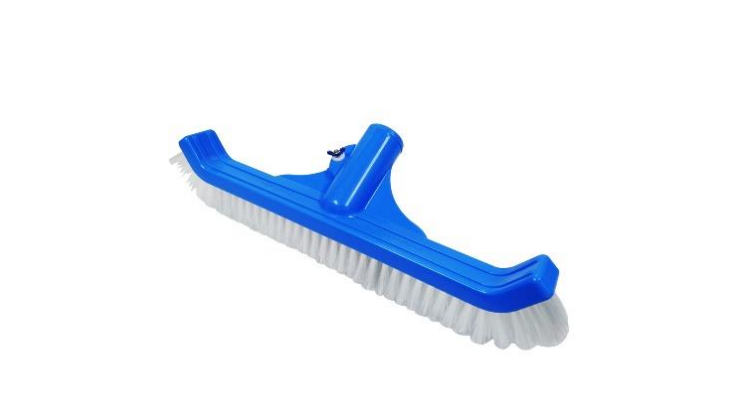
\includegraphics[width=0.60\textwidth]{imagens/escova.png}
                \caption*{Escova}
                \caption*{Fonte: \cite{benedito2024projeto}}
            \end{figure}

        \subsubsection*{Cabo de alumínio}

         \textcolor{black}{O cabo de alumínio tem a função de se encaixar nos equipamentos citados anteriormente. Está disponível em diversos tamanhos, garantindo melhor conforto e praticidade no momento do manuseio \cite{benedito2024projeto}.}

            \begin{figure}[H]
                \centering
                \caption{ }  
                \centering
                \label{fig:cont}
                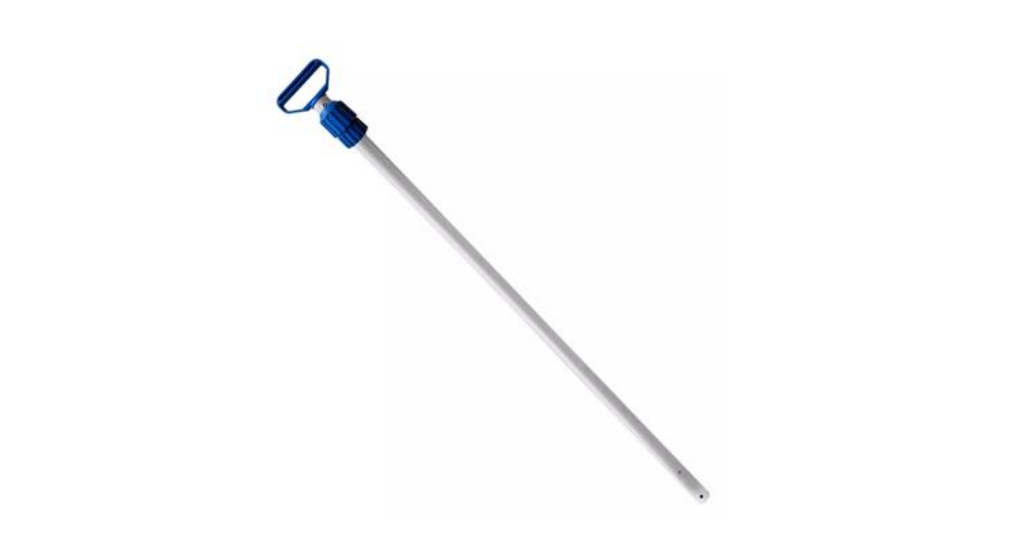
\includegraphics[width=0.60\textwidth]{imagens/cabo}.png
                \caption*{Cabo de alumínio}
                \caption*{Fonte: \cite{benedito2024projeto}}
            \end{figure}

        Portanto, é entendível que a manutenção de uma piscina envolve diversos componentes essenciais para uma limpeza eficiente. Cada componente possui um papel fundamental para garantir a circulação, filtração e tratamento adequados da água. 
        
        Esses elementos, aliados a boas práticas de operação e manutenção, constituem a base para o funcionamento eficiente do sistema. Entretanto, a eficiência desse processo não se restringe aos equipamentos mecânicos, dependendo também da aplicação correta dos procedimentos técnicos e químicos que asseguram a qualidade da água.
        
        Dessa forma, o próximo tópico abordará as normas e os procedimentos técnicos de limpeza manual, indispensáveis para a preservação da saúde do usuário.

    \subsection{NORMAS E PROCEDIMENTOS TÉCNICOS DE LIMPEZA MANUAL}

       \textcolor{black}{Segundo \cite{piscineiroProfissional}, a falta de um procedimento correto de limpeza pode acarretar sérios problemas de saúde para os usuários da piscina, como dermatite, micose e outras infecções. O tratamento deve ser constante e realizado de forma eficiente, de modo que os resultados estejam sempre em conformidade com as normas estabelecidas pela Associação Brasileira de Normas Técnicas ABNT\footnote{Associação Brasileira de Normas Técnicas, responsável por estabelecer as diretrizes de padronização para trabalhos acadêmicos no Brasil.}. De acordo com \cite{guiaTratamento}, existem diversos fatores poluentes presentes em uma piscina, como suor e urina, pelos e cabelos, óleos da pele, insetos, folhas, formação de algas, entre outros.}

       \textcolor{black}{Esses poluentes podem comprometer diretamente os parâmetros químicos da piscina, como o pH e o nível de cloro. Segundo o mesmo autor, ao realizar apenas a limpeza física, por meio de escovas ou redes, é possível remover somente a parte visível dos resíduos, como folhas, insetos e lodo. Por essa razão, torna-se necessária a aplicação de um tratamento químico eficaz, uma vez que poluentes como suor e urina se misturam à água, e os sistemas de filtragem são incapazes de removê-los completamente.}

       %Tentar inserir alguma imagem no final de algum desses três paragrafos pois esta tudo muito grande

       \textcolor{black}{É de fundamental importância que a água de uma piscina limpa atenda a determinados pré-requisitos, tais como: ausência de bactérias do grupo coliforme ou Staphylococcus aureus\footnote{Bactéria coco Gram-positiva, frequentemente encontrada na pele e nas fossas nasais humanas, responsável por infecções de gravidade variável.}, boa visibilidade do fundo, superfície livre de sujeiras e pH dentro da faixa ideal, entre 7,2 e 7,8.}

       Para que esses parâmetros sejam alcançados, é essencial que a água apresente três princípios básicos:
    
       \begin{itemize}
            \item \textbf{\textcolor{black}{Água Limpa:}} \textcolor{black}{Água transparente e sem a presença de sedimentos.}
            
            \item \textbf{\textcolor{black}{Água Balanceada:}} \textcolor{black}{Segundo todos os parâmetros prescritos, sem risco de prejudicar o banhista.}
             
            \item \textbf{\textcolor{black}{Água Saudável:}} \textcolor{black}{Livre de micro-organismos que podem vir a prejudicar o banhista.}
            
        \end{itemize}

        \begin{figure}[H]
                \centering
                \caption{ }  
            	\centering
                \label{fig:cont}
            	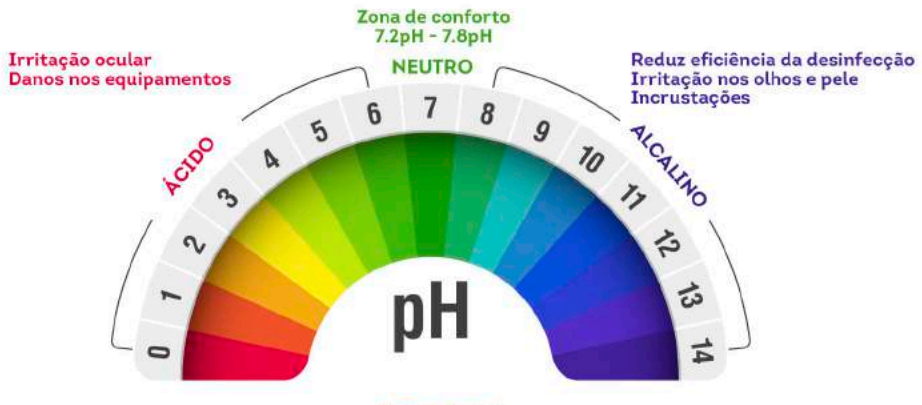
\includegraphics[width=0.48\textwidth]{imagens/medidorPh.png}
                \caption*{Faixa de pH}
            	\caption*{Fonte: \cite{guiaTratamento}}
        \end{figure}


        \textcolor{black}{Antes do processo de limpeza, é fundamental conhecer a área e o volume da piscina, a fim de determinar a quantidade adequada de produtos químicos e garantir uma higienização eficiente, sem desperdícios.}

        O cálculo da área e do volume pode variar conforme o formato da piscina, sendo possível aplicar diferentes fórmulas geométricas para cada tipo de estrutura.

        \subsubsection*{\textcolor{black}{Piscina Retangular}}
        
            \[
            A = \text{comprimento} \times \text{largura}
            \]
            \[
            V = \text{comprimento} \times \text{largura} \times \text{profundidade}
            \]
            
        \subsubsection*{\textcolor{black}{Piscina Circular}}
            \[
            A = \pi r^2
            \]
            \[
            V = \pi r^2 h
            \]
            
        \subsubsection*{\textcolor{black}{Piscina Oval (Elíptica)}}
            \[
            A = \pi \cdot \frac{a}{2} \cdot \frac{b}{2}
            \]
            \[
            V = A \cdot h
            \]
            
            \textcolor{black}{Nos casos em que a piscina possui fundo inclinado, a profundidade considerada deve ser a média entre a parte mais rasa e a mais funda:}
            \[
            h_m = \frac{h_{\text{maior}} + h_{\text{menor}}}{2}
            \]
            

        \textcolor{black}{Segundo \cite{tccSilva}, o processo de limpeza é semelhante ao empregado em indústrias, como nas estações de tratamento de água, e segue uma sequência composta por cinco etapas principais:}

        \begin{itemize}
            \item \textbf{\textcolor{black}{Oxidação:}} \textcolor{black}{tapa em que ocorre a adição de cloro, com o objetivo de oxidar metais, como ferro e manganês, facilitando a remoção da matéria orgânica.}
            
            \item \textbf{\textcolor{black}{Coagulação e Floculação:}} \textcolor{black}{consiste na adição de sulfato de alumínio e, ocasionalmente, cloreto férrico, para promover o desequilíbrio das partículas. Em seguida, a circulação da água possibilita a formação dos flocos.}
             
            \item \textbf{\textcolor{black}{Decantação:}} \textcolor{black}{ocorre quando as partículas coaguladas e floculadas se depositam no fundo da piscina, em razão da circulação lenta do fluido. Dependendo do produto utilizado, essa etapa pode durar aproximadamente seis horas.}

            \item \textbf{\textcolor{black}{Filtração:}} \textcolor{black}{responsável pela retenção das impurezas acumuladas nas etapas anteriores, geralmente realizada por meio de um filtro de areia.}

            \item \textbf{\textcolor{black}{Correção de pH:}} \textcolor{black}{envolve a análise e o ajuste do pH da água, normalmente com o auxílio de um medidor, procedimento essencial para evitar a deterioração das tubulações e dos equipamentos, bem como prevenir possíveis doenças em banhistas.}
            
        \end{itemize}

        \textcolor{black}{Em virtude do exposto, torna-se evidente que a aplicação correta dos procedimentos técnicos estabelecidos é indispensável para a manutenção da qualidade da água. Nesse contexto, a precisão e a segurança exigidas pelo processo dependem diretamente da seleção e do manuseio adequado dos produtos químicos, tema que será abordado na seção seguinte.}


    \subsection{PRODUTOS QUÍMICOS E ACESSÓRIOS USADOS NA LIMPEZA DE PISCINAS}

        \textcolor{black}{O tratamento adequado e corretamente executado durante a limpeza de uma piscina, tanto físico quanto químico, é essencial para assegurar a qualidade da água e prevenir infecções ou doenças de origem hídrica. Dessa forma, é fundamental compreender quais produtos utilizar, como aplicá-los corretamente e qual o método mais eficiente para a realização do tratamento físico.}

        O principal objetivo desta seção é apresentar os produtos e ferramentas recomendados para assegurar a qualidade da água e preservar a saúde dos usuários.

        \begin{itemize}
        
            \item \textbf{\textcolor{black}{Precedimento Químico:}} \textcolor{black}{segundo \cite{guiaTratamento}, o procedimento químico compreende todas as etapas relacionadas à adição de substâncias químicas à água, com o objetivo de assegurar sua qualidade e prevenir riscos à saúde dos banhistas. Esses produtos são responsáveis por ajustar a alcalinidade e o pH, além de promover a desinfecção da água por meio da eliminação de micro-organismos e bactérias, utilizando cloro e outros compostos destinados ao controle dos parâmetros químicos.}

                \begin{figure}[H]
                    \centering
                    \caption{ }  
                	\centering
                    \label{fig:cont}
                	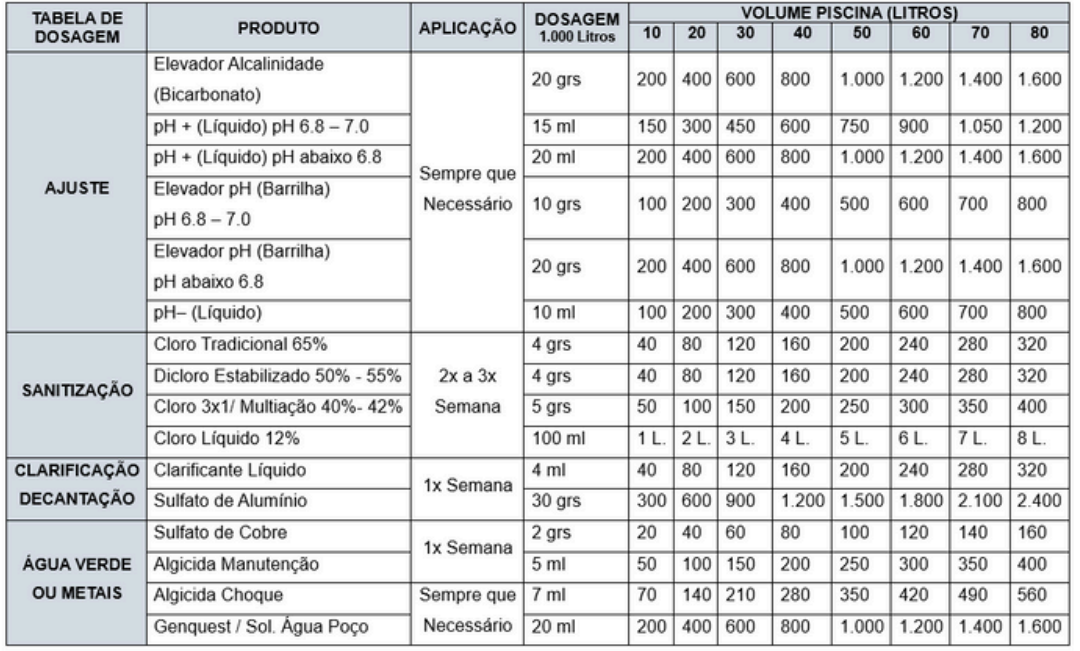
\includegraphics[width=1.00\textwidth]{imagens/tabelaProdutos.png}
                    \caption*{Tabela de Dosagem de Produtos}
                	\caption*{Fonte: \cite{guiaTratamento}}
                \end{figure}
    
                \begin{itemize}
    
                    \item \textbf{\textcolor{black}{Elevador de Alcalinidade:}} \textcolor{black}{a alcalinidade da água está relacionada à sua capacidade de neutralizar ácidos, atuando como uma barreira química que mantém o pH estável. O produto utilizado tem como finalidade elevar a alcalinidade até o nível ideal, que deve permanecer entre 80 e 120 ppm.}
    
                    \item \textbf{\textcolor{black}{Barrilha, Elevador de pH, pH+:}} \textcolor{black}{pProdutos de composição alcalina, empregados para elevar o pH da água quando este se encontra abaixo do nível ideal.}
    
                    \item \textbf{\textcolor{black}{Redutor de pH, pH-:}} \textcolor{black}{produtos de composição ácida que têm a função de diminuir o pH da água.}
    
                    \item \textbf{\textcolor{black}{Hipoclorito de Sódio, Cloro, Dicloro, Multiação 3x1:}} \textcolor{black}{agentes sanitizantes, cuja finalidade é eliminar micro-organismos presentes na água, garantindo sua desinfecção e potabilidade.}
    
                    \item \textbf{\textcolor{black}{Sulfato de Alumínio, Clarificantes:}} \textcolor{black}{provocam o processo de decantação, no qual as partículas de impurezas são aglomeradas e conduzidas ao fundo da piscina, facilitando as etapas subsequentes de aspiração e filtração.}
    
                    \item \textbf{\textcolor{black}{Sulfato de Cobre, Algicida:}} \textcolor{black}{utilizados, quando a piscina apresenta coloração esverdeada, esses produtos atuam na eliminação de algas e na remoção de lodo, restabelecendo a qualidade visual e sanitária da água.}
    
                    \item \textbf{\textcolor{black}{Genquest, Solução Água de poço:}} \textcolor{black}{empregados para remover manchas e colorações decorrentes da presença de metais dissolvidos na água, contribuindo para a manutenção do aspecto estético e da pureza visual do reservatório.}
    
                \end{itemize}
                
            \item \textbf{\textcolor{black}{Medição de Parâmetros e Ajuste do pH:}} \textcolor{black}{para a avaliação dos parâmetros da água, utilizam-se estojos de análise específicos para cada variável a ser monitorada. O ajuste adequado desses parâmetros é fundamental para garantir um processo de tratamento eficiente e seguro.}

            \begin{figure}[H]
                    \centering
                    \caption{ }  
                	\centering
                    \label{fig:cont}
                	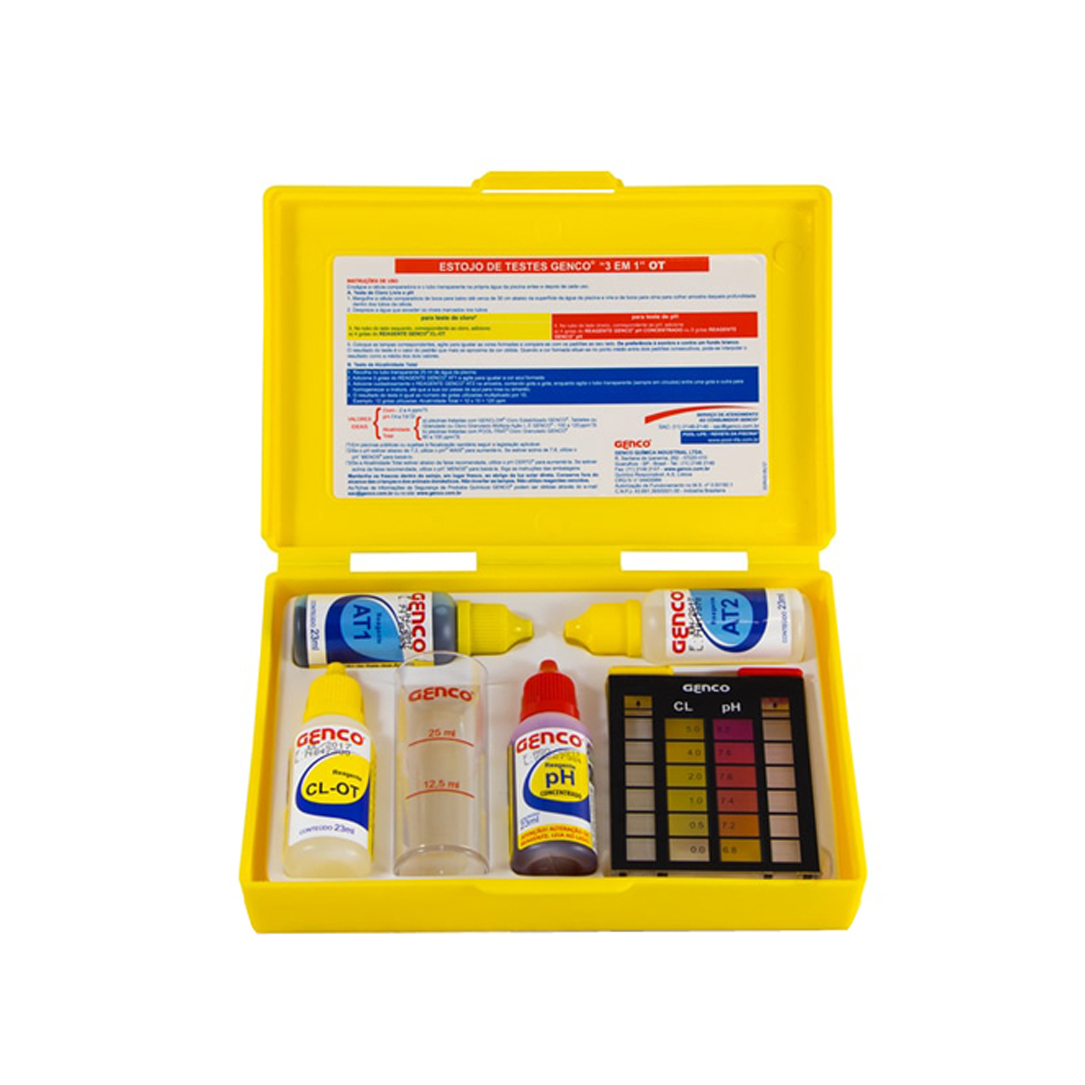
\includegraphics[width=0.48\textwidth]{imagens/estojoMedidor.png}
                    \caption*{Estojo para Análise de Parâmetros}
                	\caption*{Fonte: \cite{gencoEmpresa}}
            \end{figure}

            %Colocar imagens de medidor
            \textcolor{black}{Os produtos a serem aplicados variam conforme os resultados obtidos nas análises químicas da água. Caso o pH apresente valores inferiores a 7,0, deve-se utilizar o elevador de pH ou barrilha. Se a alcalinidade estiver abaixo do nível ideal, recomenda-se a aplicação do elevador de alcalinidade. Por fim, quando o nível de cloro estiver reduzido, é necessário adicionar cloro líquido ou granulado, conforme indicado na tabela apresentada anteriormente.}

            \item \textbf{\textcolor{black}{Limpeza química:}} \textcolor{black}{Com base nas informações apresentadas, compreende-se que a turbidez da água, caracterizada pela presença de partículas em suspensão, é um dos principais indicadores da necessidade de tratamento químico. Para corrigir esse problema, recomenda-se o uso de um decantador, que aglomera as partículas e as leva ao fundo da piscina, permitindo sua posterior aspiração.}
            
            \begin{itemize}
                \item \textbf{\textcolor{black}{Clarificação:}} \textcolor{black}{utilizada quando a água está opaca e sem brilho; realiza-se com produtos clarificantes específicos.}
                
                \item \textbf{\textcolor{black}{Floculação ou decantação:}} \textcolor{black}{aplicadas quando a água se encontra turva ou suja; para isso, adiciona-se floculante líquido ou decantador em pó (geralmente, sulfato de alumínio).}
            \end{itemize}

            Após a aplicação dos produtos, recomenda-se aguardar entre 6 e 12 horas antes de iniciar o processo de aspiração do fundo da piscina.

            %\textcolor{red}{colocar imagens de piscinas verdes e opacas, no final de tudo ou após a citação de cada uma}
            
        \end{itemize}

        \textcolor{black}{Com todos os dados e informações apresentados, é possível compreender o processo necessário para realizar uma limpeza eficiente de piscina. Entretanto, esse procedimento pode se mostrar complexo para algumas pessoas, motivo pelo qual surgem alternativas tecnológicas, especialmente por meio da automação residencial, que será abordada na próxima seção.}
         
   
\section{FUNDAMENTOS DA AUTOMAÇÃO RESIDENCIAL}

    Após compreender os aspectos estruturais e os métodos tradicionais de manutenção de piscinas, torna-se necessário examinar os princípios da automação residencial, uma vez que o sistema proposto se insere nesse contexto tecnológico. Este tópico aborda a evolução histórica da automação aplicada ao ambiente doméstico, seus conceitos técnicos, componentes essenciais e protocolos de comunicação, que viabilizam o controle remoto e inteligente de diferentes dispositivos. Essa fundamentação permite compreender como as tecnologias emergentes podem ser aplicadas para aprimorar processos cotidianos, incluindo a manutenção automatizada de piscinas.

    \textcolor{black}{A automação residencial consiste na integração de sistemas tecnológicos voltados ao controle e à otimização de funções domésticas, como segurança, iluminação, climatização e comunicação. Essa integração, também conhecida como domótica, tem como propósito aprimorar o conforto, a segurança e a eficiência energética das residências \cite{automacaoResidencialCap1}.}

    \textcolor{black}{O principal objetivo da automação residencial é proporcionar comodidade e segurança aos usuários, por meio da operação remota e da integração de dispositivos inteligentes \cite{automacaoTecnologiaPraticidade}}

    \textcolor{black}{A automação residencial é composta por um conjunto de benefícios fundamentais que estruturam o conceito de casa inteligente. Entre seus principais pilares, destacam-se:}

    \begin{itemize}
        \item \textbf{\textcolor{black}{Conforto:}} \textcolor{black}{sendo um dos pilares centrais, tem como objetivo facilitar as tarefas cotidianas. A automação proporciona maior comodidade ao usuário, permitindo o controle remoto de lâmpadas, ar-condicionados, sistemas de irrigação, entre outros \cite{automacaoTecnologiaPraticidade}.}
        
        \item \textbf{\textcolor{black}{Segurança:}} \textcolor{black}{a integração de câmeras, fechaduras eletrônicas e sensores de luz e presença torna a segurança um dos principais benefícios da automação. Isso possibilita o monitoramento remoto da residência, reforçando os aspectos de proteção, praticidade e conforto \cite{automacaoTecnologiaPraticidade}.}
        
        \item \textbf{\textcolor{black}{Economia:}} \textcolor{black}{a automação também contribui para o uso racional de energia, por meio de sistemas que desligam lâmpadas automaticamente e ajustam a climatização conforme a necessidade. Dessa forma, evita-se o desperdício e promove-se maior eficiência energética \cite{automacaoTecnologiaPraticidade}.}
        
    \end{itemize}

    \textcolor{black}{Para que a automação funcione de forma adequada, é necessário o uso de dispositivos com conectividade, acesso à internet e um sistema central de controle capaz de realizar a coleta e troca de informações entre os equipamentos.}

    Praticamente todos os aparelhos eletrônicos que possuem algum tipo de acionamento podem ser automatizados, como sistemas de iluminação, portões, climatização e segurança. Esses dispositivos são conectados a uma central de controle, que pode ser acessada por meio de um display touch\footnote{O display touch é uma superfície sensível ao toque que permite a interação direta do usuário}, localizado na própria central, aplicativos para smartphones ou comandos de voz \cite{automacaoTecnologiaPraticidade}.

    \subsection{HISTÓRICO E EVOLUÇÃO DA AUTOMAÇÃO RESIDENCIAL}

        \textcolor{black}{Embora recente, a automação residencial tem evoluído rapidamente. Na década de 1970, surgiram nos Estados Unidos os primeiros módulos inteligentes baseados em transmissão de dados pela rede elétrica doméstica, utilizando a tecnologia PLC \textit{(Power Line Communication)} \cite{automacaoResidencialCap1}.}

        \textcolor{black}{O avanço da informática e da internet possibilitou a criação de sistemas residenciais inteligentes, capazes de monitorar e controlar equipamentos à distância, consolidando o conceito moderno de casa conectada.}

        A seguir, apresenta-se uma tabela que ilustra a evolução de algumas das principais tecnologias utilizadas na automação residencial:

        \begin{table}[H]
            \centering
            \renewcommand{\arraystretch}{1.3}
            \setlength{\tabcolsep}{10pt}
            \begin{tabular}{lccccc}
            \hline
            \textbf{Tecnologia} & \textbf{2003} & \textbf{2004} & \textbf{2005} & \textbf{2006} & \textbf{2015(*)} \\
            \hline
            Cabeamento estruturado & 42\% & 61\% & 49\% & 53\% & 80\% \\
            Monitoramento de segurança & 18\% & 28\% & 29\% & 32\% & 81\% \\
            Multiroom audio & 9\% & 12\% & 15\% & 16\% & 86\% \\
            Home Theater & 9\% & 8\% & 11\% & 12\% & 86\% \\
            Controle de iluminação & 1\% & 2\% & 6\% & 8\% & 75\% \\
            Automação integrada & 0\% & 2\% & 6\% & 6\% & 70\% \\
            Gerenciamento de energia & 1\% & 5\% & 11\% & 11\% & 62\% \\
            \hline
            \end{tabular}
            \caption{Evolução das tecnologias de automação residencial ao longo dos anos.}
            \label{tab:tecnologias-automacao}

            \vspace{0.5em}
            \small
            \textbf{Fonte:} \cite{automacaoResidencialCap1}.\\
        \end{table}

        \textcolor{black}{Dessa forma, ao compreender a evolução histórica e o crescimento das tecnologias aplicadas à automação residencial, torna-se evidente a importância de conhecer os fundamentos técnicos que sustentam esse campo.}

        No próximo tópico, serão abordados alguns dos principais conceitos e componentes que compõem a base dos sistemas automatizados, como controladores, sensores, atuadores e protocolos de comunicação. Esses elementos são essenciais para o entendimento do funcionamento e da integração entre os dispositivos que possibilitam a automação em ambientes residenciais.


    \subsection{CONCEITOS TÉCNICOS DE AUTOMAÇÃO RESIDENCIAL}
    
       \textcolor{black}{Tecnicamente denominada domótica, a automação residencial tem como principal objetivo acionar, monitorar, integrar e controlar diferentes tipos de variáveis ou cargas de uma residência, como iluminação, climatização, áudio e vídeo, com o intuito de gerar eficiência, comodidade e segurança para o usuário \cite{oliveira2019domotica}.}

       No Brasil, o termo mais comumente utilizado é automação residencial, traduzido diretamente da expressão americana \textit{home automation}. Contudo, essa tradução não abrange totalmente o significado do termo domótica. O uso de novas tecnologias no país vem crescendo exponencialmente; entretanto, o mercado da construção civil ainda não acompanha o mesmo ritmo de evolução tecnológica observado em setores como o automotivo, que já utiliza amplamente tecnologias embarcadas\footnote{Computador especializado, composto por hardware e software, que executa uma função dedicada dentro de um sistema maior} \cite{hipolito2018automaccao}.

       \textcolor{black}{De acordo com \cite{accardi2012automaccao}, a forma como os componentes se comunicam está diretamente relacionada à arquitetura adotada, que pode ser centralizada ou descentralizada.}

       Em uma arquitetura centralizada, todos os componentes do sistema respondem a um único dispositivo, que por sua vez, deve ter uma alta inteligência e desempenho.

        \begin{figure}[H]
                \centering
                \caption{ }  
                \centering
                \label{fig:cont}
                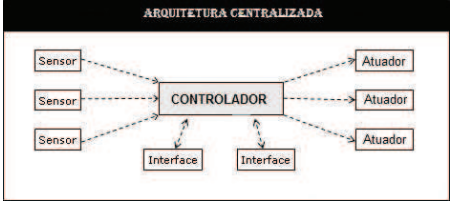
\includegraphics[width=0.53\textwidth]{imagens/arquiteturaCentralizada.png}
                \caption*{Arquitetura centralizada}
                \caption*{Fonte: \cite{hipolito2018automaccao}}
        \end{figure}

       \textcolor{black}{Na arquitetura descentralizada, diversos controladores coexistem e se comunicam entre si por meio de um barramento de dados\footnote{Refere-se a um sistema onde a comunicação e a coordenação entre os componentes são distribuídas, sem depender de uma autoridade ou ponto central}, compartilhando o controle dos dispositivos interconectados..}

        \begin{figure}[H]
                \centering
                \caption{ }  
                \centering
                \label{fig:cont}
                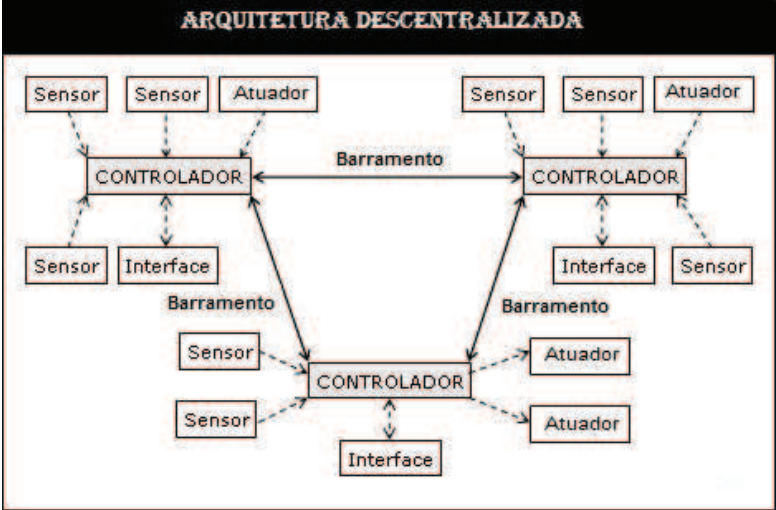
\includegraphics[width=0.53\textwidth]{imagens/arquiteturaDescentralizada.png}
                \caption*{Arquitetura descentralizada}
                \caption*{Fonte: \cite{hipolito2018automaccao}}
         \end{figure}

       \textcolor{black}{Para que toda a integração dos sistemas ocorra de forma eficiente, é necessário compreender alguns conceitos técnicos fundamentais, que possibilitam a execução bem-sucedida das funções automatizadas.}

       Nas seções seguintes, serão apresentados esses conceitos e componentes, essenciais para o entendimento do funcionamento da automação residencial.

       \subsubsection{COMPONENTES BÁSICOS}

        \textcolor{black}{A automação residencial tem seu funcionamento composto por diversos componentes, que variam desde sensores simples até centrais complexas de automação. A seguir, são apresentados alguns dos principais elementos que compõem essa estrutura:}

            \begin{itemize}
                \item \textbf{\textcolor{black}{Camadas de dispositivos:}} \textcolor{black}{(1)~Sensores: Segundo \cite{hipolito2018automaccao}, um sensor pode ser definido como um dispositivo sensível ao ambiente no qual está inserido, capaz de detectar alterações em variáveis como temperatura, luminosidade ou movimento. (2)~Atuadores: são componentes eletromecânicos acionados pelo sistema para executar uma função específica, como ativar uma sirene, lâmpada, fechadura magnética, motor ou válvula. (3)~Controladores: têm como função monitorar os parâmetros coletados pelos sensores e, de acordo com os dados obtidos, acionar o respectivo atuador vinculado. Podem possuir interfaces próprias ou fazer parte de grandes centrais de controle. (4)~Interfaces: dispositivos que permitem ao usuário interagir com o sistema automatizado, como aplicativos móveis, painéis digitais ou páginas web \cite{accardi2012automaccao}.}
                
                \item \textbf{\textcolor{black}{Camada de comunicação/rede:}} \textcolor{black}{Segundo \cite{accardi2012automaccao}, a camada de comunicação, também chamada de protocolo, “é um acordo entre as partes que se comunicam, estabelecendo como se dará a comunicação”. Assim, entende-se que um protocolo é, em resumo, o conjunto de regras e padrões utilizados para que diferentes dispositivos possam se comunicar entre si.}
                
                Entre os principais protocolos empregados na automação residencial, destacam-se: Ethernet, X-10, HomePNA e Wi-Fi. Alguns desses protocolos foram desenvolvidos especificamente para a automação residencial, enquanto outros foram adaptados de aplicações industriais e comerciais.
                
                \item \textbf{\textcolor{black}{Camada de controle/automação lógica:}} \textcolor{black}{A camada de controle, também chamada de central de automação, pode ser considerada o “cérebro” do sistema, sendo responsável por gerenciar todos os dispositivos conectados. Ela processa as informações de entrada e saída e executa as ações necessárias conforme as instruções programadas.}
                
                A configuração da central pode ser realizada por meio de um software dedicado, acessado através de um computador ou dispositivo móvel. Essa central é escalável\footnote{Descreve algo que pode crescer ou ser aumentado em magnitude, seja física ou figurativamente}, permitindo que novos dispositivos sejam adicionados ao sistema de forma contínua, conforme a necessidade de expansão.
        
            \end{itemize}
    

    \textcolor{black}{Diante de todos os dados e fundamentos apresentados, fica evidente que a automação residencial encontra-se em constante evolução, impulsionada pela integração de sensores, controladores, motores e protocolos de comunicação. Esses elementos, quando aplicados corretamente, possibilitam o desenvolvimento de sistemas inteligentes, capazes de automatizar e otimizar tarefas rotineiras.}

    Nesse contexto, o próximo capítulo abordará o desenvolvimento de um sistema automatizado de limpeza de piscinas, aplicando na prática os conceitos estudados e demonstrando como a integração entre hardware e software pode oferecer uma solução segura, eficiente e inovadora para a manutenção de piscinas residenciais.

\section{FERRAMENTAS UTILZIADAS PARA AUTOMAÇÃO}

    \textcolor{blue}{Esta seção tem como objetivo fundamentar as principais ferramentas e tecnologias empregadas no desenvolvimento do sistema de automação, abrangendo desde os componentes físicos de hardware até os frameworks de software e as metodologias aplicadas à engenharia de projetos.}

    \subsection{COMPONENTES FÍSICOS E DE CONTROLE (HARDWARE)}

        \textcolor{blue}{O sistema de automação requer hardware dedicado tanto para o processamento central quanto para a interação com o ambiente físico.}

        \subsubsection*{Raspberry Pi}
        